\documentclass[
    12pt,
    article,
    oneside,
    a4paper,
    english,
    brazil
]{abntex2}

\usepackage[utf8]{inputenc}
\usepackage[T1]{fontenc}
\usepackage{lmodern}
\usepackage{indentfirst}
\usepackage[rgb]{xcolor}
\usepackage{graphicx}
\usepackage{microtype}
\usepackage{longtable}
\usepackage{booktabs}
\usepackage{array}
\usepackage{amsmath}
\usepackage{amsfonts}
\usepackage{amssymb}
\usepackage{caption}
\usepackage{enumitem}


% --- Controle de Posição de Imagens ---
\usepackage{float}
\usepackage[section]{placeins} 

% Forçar todas as figuras a usarem o posicionamento [H]
\floatplacement{figure}{H}
\floatplacement{table}{H}

% --- Pandoc Fixes ---
\ifdefined\pandocbounded
\else
  \newcommand{\pandocbounded}[1]{#1}
\fi

% --- Forçar Centralização de Todas as Figuras ---
\makeatletter
\g@addto@macro\@floatboxreset\centering
\makeatother

\usepackage[alf]{abntex2cite}

\definecolor{blue}{RGB}{41,5,195}
\hypersetup{
    colorlinks=true,
    linkcolor=blue,
    citecolor=blue,
    urlcolor=blue
}

\setlrmarginsandblock{3cm}{2cm}{*}
\setulmarginsandblock{3cm}{2cm}{*}
\checkandfixthelayout

\titulo{Predição de Risco de Diabetes tipo II via Redes Neurais Profundas: Um Estudo com o Dataset BRFSS 2015}
\autor{
  Antonio Uriel Ewerton do Vale \\
  Brendon Nicholas de Oliveira Silva \\
  Daniel Rocha da Silva \\
  Jose Francisco da Silva Neto \\
  Maria Luiza de Sousa Lima
}
\local{Brasil}
\data{2026}

\renewcommand{\maketitle}{
    \begin{center}
        {\ABNTEXchapterfont\Large\imprimirtitulo} \\
        \vspace{1cm}
        {\imprimirautor} \\
        \vspace{0.5cm}
        \imprimirlocal, \imprimirdata
    \end{center}
    \vspace{1cm}
}

\begin{document}
\selectlanguage{brazil}
\frenchspacing

\maketitle

\section{Resumo (Abstract)}\label{resumo-abstract}

\textbf{Português:} Este trabalho investiga a capacidade de redes neurais artificiais do tipo Perceptron Multicamada (MLP) para estimar o risco de desenvolver diabetes tipo 2. Utilizando 253.680 entradas do \emph{Behavioral Risk Factor Surveillance System} (BRFSS) de 2015, aplicou-se um classificador binário local. A abordagem envolve engenharia de atributos, normalização dos dados e a criação de um modelo de seis camadas ocultas. O protótipo atingiu 85,19\% de acurácia e 0,82 de AUC-ROC em 130,64 segundos de treino num AMD Ryzen 7. Foram exploradas a aplicabilidade do protótipo para triagens, a contribuição dos fatores de risco via a sua importância por permutação e as fragilidades da modelagem baseada em dados autorreportados versus dados laboratoriais.

\textbf{English:} This work investigates the capacity of Multilayer Perceptron (MLP) artificial neural networks to estimate the risk of developing type 2 diabetes. Using 253,680 entries from the 2015 Behavioral Risk Factor Surveillance System (BRFSS), a local binary classifier was applied. The approach involves feature engineering, data normalization, and the creation of a model with six hidden layers. The prototype achieved 85.19% accuracy and a 0.82 AUC-ROC in 130.64 seconds of training on an AMD Ryzen 7. The prototype's applicability for screening, the contribution of risk factors via permutation importance, and the weaknesses of modeling based on self-reported data versus laboratory data were explored.

\textbf{Keywords:} Diabetes Prediction, Deep Learning, MLP, Healthcare AI, BRFSS, Predictive Analytics.


\newpage

\section{Introdução}
O diabetes tipo 2 é uma condition caracterizada pela resistência à insulina e pela hiperglicemia. Como os casos da doença têm crescido rapidamente, sobretudo em países de média e baixa renda, conseguir identificá-la de forma precoce na população tornou-se uma necessidade urgente [4].
O uso de técnicas de \emph{Deep Learning} permite explorar grandes bases de dados à escala populacional. Este artigo avalia se redes MLP treinadas com dados recolhidos em inquéritos populacionais são capazes de indentificar pessoas em grupos de risco [3], funcionando assim como o instigador de uma breve triagem de saúde digital a baixo custo.
\section{Problema de pesquisa}
Dados populacionais apresentam as suas próprias limitações pois facilmente são permeáveis à subjetividade e ao ruído dos dados auto-reportados. Assim, este trabalho questiona em que medida uma rede neural profunda, amplamente paralelizada, consegue extrair padrões robustos a partir de variáveis subjetivas e providenciar respostas sobre o risco de diabetes que possam servir de alerta para uma triagem.

\section{Metodologia e ambiente de teste}\label{metodologia-e-ambiente-de-teste}
\subsection{Infraestrutura de hardware}\label{infraestrutura-de-hardware}
Testes correm localmente num sistema reforçado por um processador AMD Ryzen 7 7700X (16 vCPUs a 5,57 GHz), 32 GB de memória RAM DDR5 a 6000 MHz, uma placa gráfica AMD Radeon RX 7600 XT e Fedora Linux 44 Workstation Edition.

\subsection{O conjunto de dados (Dataset)}\label{o-conjunto-de-dados-dataset}
O \emph{Diabetes Health Indicators Dataset} é uma versão tratada dos dados do BRFSS 2015 disponível no Kaggle [1]. A base de dados total conta com 253.680 registros, dos quais 20\% (50.736 amostras) foram reservados para o conjunto de testes. Para garantir a representatividade, a divisão foi realizada via amostragem aleatória estratificada, preservando a proporção da variável alvo em ambos os subconjuntos. O modelo processa 21 variáveis de entrada que cobrem quatro dimensões principais da saúde: 

\begin{itemize}
    \item \textbf{Demografia:} Idade (\texttt{Age}), sexo (\texttt{Sex}), nível de escolaridade (\texttt{Education}) e faixa de rendimento (\texttt{Income}).
    \item \textbf{Biometria:} Índice de Massa Corporal (\texttt{BMI}).
    \item \textbf{Estilo de vida:} Tabagismo (\texttt{Smoker}), prática de atividade física (\texttt{PhysActivity}), consumo diário de frutas e vegetais (\texttt{Fruits}, \texttt{Veggies}) e consumo excessivo de álcool (\texttt{HvyAlcoholConsump}).
    \item \textbf{Histórico clínico e autopercepção:} Avaliação da saúde geral (\texttt{GenHlth}), saúde física (\texttt{PhysHlth}), histórico de hipertensão arterial (\texttt{HighBP}), colesterol alto (\texttt{HighChol}), além de outros indicadores como histórico de AVC, doenças cardíacas e dificuldade de locomoção (\texttt{DiffWalk}).
\end{itemize}

\subsection{Engenharia de atributos e normalização}\label{engenharia-de-atributos-e-normalizauxe7uxe3o}
Para explora a influência da interação entre os fatores de risco, são construídas três variáveis derivadas. A variável \texttt{BMI\_Age} associa o IMC às faixas etárias do indivíduo. A variável \texttt{HighBP\_HighChol} funde os dois fatores de risco com maior implicação na gênese da DC para representar o risco cardiovascular acumulado. Finalmente, a variável \texttt{GenHlth\_PhysHlth} explora a saúde subjetiva e objetiva da amostra, estabelecendo uma relação entre a autoperceção da saúde geral e os dias reportados de incapacidade física.

\section{Arquitetura da rede neural proposta}\label{arquitetura-da-rede-neural-proposta}
O classificador é uma rede sequencial de seis camadas ocultas implementada em TensorFlow [2], com cerca de 1,8 milhão de parâmetros treináveis. As duas primeiras camadas possuem 1024 neurônios cada e têm por objetivo capturar as relações iniciais do espaço de características [5]. As camadas subsequentes realizam uma compressão progressiva dos dados para 512, 256, 128 e 64 neurônios, extraindo os fatores latentes mais importantes para a tarefa de classificação binária. Para normalizar os gradientes e impedir o sobreajuste, empregou-se \emph{BatchNormalization} após cada camada oculta, além de camadas de \emph{Dropout} com taxas decrescentes entre 40\% e 20\%. A convergência foi auxiliada pelo \emph{callback ReduceLROnPlateau}, que diminui a taxa de aprendizado ao detectar que a perda estabilizou.

\section{Resultados e análise}\label{resultados-e-anuxe1lise}
O treinamento durou 130, 64 segundos e foi interrompido na 36ª época através do mecanismo de \emph{Early Stopping}.

\subsection{Resumo dos indicadores de desempenho}\label{resumo-dos-indicadores-de-desempenho}
As métricas alcançadas pelo classificador MLP no conjunto de teste são apresentadas na Tabela 1.

\begin{longtable}[]{@{}lll@{}}
\toprule
Métrica & Valor Obtido & Definição \\
\midrule
\endhead
\textbf{Acurácia Global} & 85,19\% & Fração de predições corretas total. \\
\textbf{AUC-ROC} & 0,8222 & Capacidade de distinguir entre as classes. \\
\textbf{Average Precision} & 0,4600 & Precisão média na classe minoritária. \\
\textbf{Latência Média} & 745,21 ms & Tempo médio de resposta por requisição. \\
\textbf{Throughput} & 39,46 req/s & Requisições processadas por segundo. \\
\bottomrule
\caption{Métricas de desempenho do classificador e da API sob estresse (30 conexões).}
\end{longtable}


Para validar a escalabilidade da solução e o comportamento da API em cenários de concorrência, submeteu-se a aplicação \emph{diabetes-app} a um teste de estresse utilizando a ferramenta \texttt{autocannon}. 

O cenário de teste foi configurado com os seguintes parâmetros:
\begin{itemize}
    \item \textbf{Concorrência:} 30 conexões simultâneas mantidas constante.
    \item \textbf{Duração:} 20 segundos de execução contínua.
    \item \textbf{Método:} HTTP POST, com o corpo da requisição formatado como \texttt{application/x-www-form-urlencoded}, replicando fielmente o comportamento esperado da interface web do usuário.
\end{itemize}

Os resultados obtidos indicam que, sob estas condições de carga, a aplicação apresentou uma latência média de 745,21 ms e um \emph{throughput} (taxa de transferência) de 39,46 requisições por segundo. 

É importante notar que, embora a inferência isolada do modelo de rede neural ocorra em tempo inferior a 25 ms, o tempo total de resposta de 745,21 ms reflete o \emph{overhead} da infraestrutura do servidor web, o processamento de serialização dos dados e a contenção de recursos sob concorrência. Estes dados demonstram a capacidade de escalabilidade do protótipo, ao mesmo tempo que evidenciam a necessidade de futuras otimizações de \emph{backend} para suportar picos de tráfego intensos.


\subsection{Convergência e aprendizado}\label{converguxeancia-e-aprendizado}

\begin{figure}
\centering
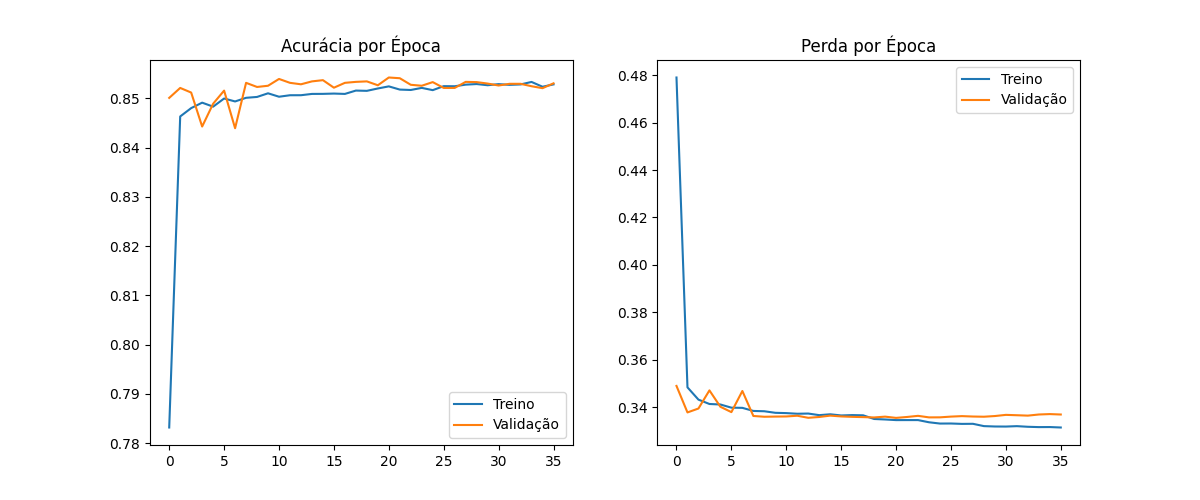
\includegraphics[width=12cm, keepaspectratio]{history_plot.png}
\caption{Variação da acurácia e da função de perda ao longo das épocas de treinamento.}
\end{figure}
O desempenho do modelo durante o treinamento (Figura 1) evidencia uma diminuição da função de perda e convergência da acurácia desde as primeiras épocas. A proximidade entre as curvas de treino e de validação sugere que os mecanismos de regularização evitaram o sobreajuste durante o processo.


\subsection{Desempenho e matriz de confusão}\label{desempenho-e-matriz-de-confusao}
\begin{figure}
\centering
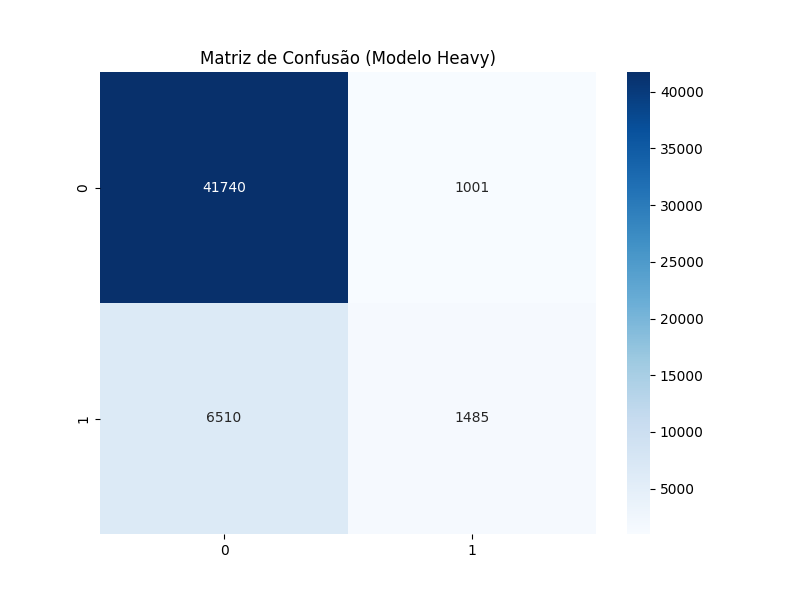
\includegraphics[width=10cm, keepaspectratio]{confusion_matrix.png}
\caption{Matriz de confusão obtida na avaliação sobre o conjunto de teste.}
\end{figure}
A matriz de confusão (Figura 2) revela que o modelo apresenta maior taxa de sucesso na identificação de indivíduos saudáveis (verdadeiros negativos), reduzindo a geração de falsos positivos. Os erros de classificação estão concentrados na classe de risco, comportamento que se alinha ao desequilíbrio da base de dados epidemiológica original. Esta é uma indicação de que o modelo deve ser utilizado apenas como um rastreador de triagem.
\subsection{Exploração das Curvas ROC e Precision-Recall}\label{exploracao-das-curvas-roc-e-precision-recall}
\begin{figure}
\centering
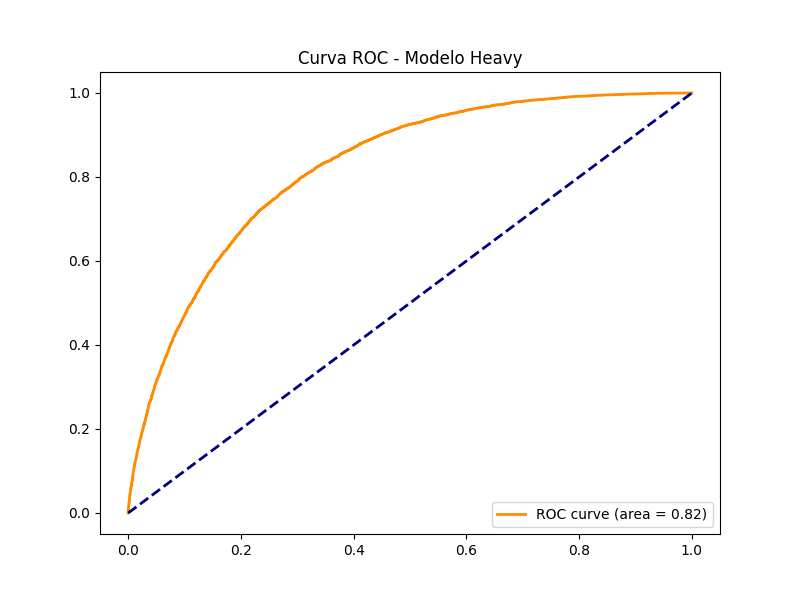
\includegraphics[width=10cm, keepaspectratio]{roc_curve.png}
\caption{Curva ROC do modelo avaliado.}
\end{figure}
\begin{figure}
\centering
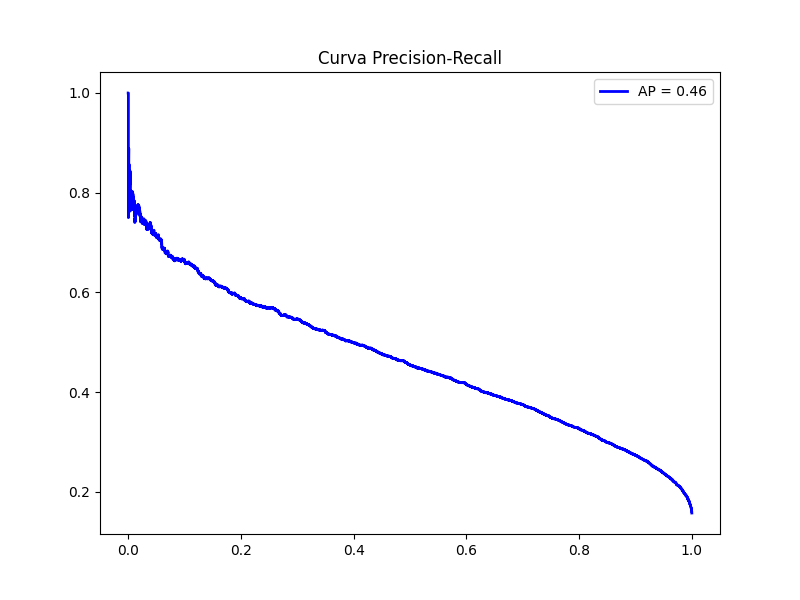
\includegraphics[width=10cm, keepaspectratio]{precision_recall_curve.png}
\caption{Curva Precision-Recall relativa \`a classe positiva.}
\end{figure}
O valor de AUC-ROC foi de 0, 82 (Figura 3). A curva Precision-Recall (Figura 4) evidencia a atua\c{c}\~ao do classificador perante o desiquil\'ibrio das amostras, uma vez que o incremento da sensibilidade (recall) provoca a perda da precis\~ao, situa\c{c}\~ao que \'e de esperar em ferramentas de rastreio populacional.
\subsection{Interpretabilidade e importância de atributos}\label{interpretabilidade-e-importancia-de-atributos}
\begin{figure}
\centering
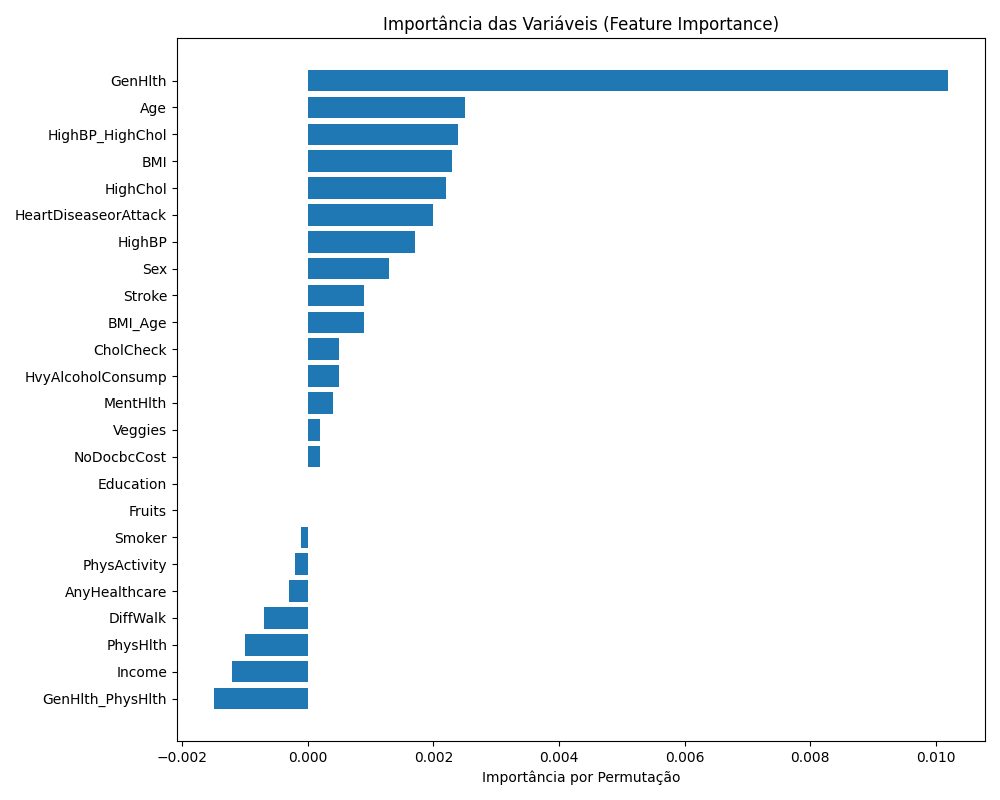
\includegraphics[width=12cm, keepaspectratio]{feature_importance.png}
\caption{Import\^ancia dos atributos calculada pelo m\'etodo de permuta\c{c}\~ao.}
\end{figure}
A import\^ancia por permuta\c{c}\~ao (Figura 5) aponta para as vari\'aveis mais determinantes nas predi\c{c}\~oes da rede neural. A perce\c{c}\~ao do estado geral de sa\'ude (\texttt{GenHlth}) destacou-se isoladamente como o fator de maior peso. Em seguida, a idade (\texttt{Age}) e o risco cardiovascular acumulado, representado pela vari\'avel sint\'etica \texttt{HighBP\_HighChol}, mostraram forte relev\^ancia para o modelo. A vari\'avel \texttt{BMI\_Age} apresentou um impacto positivo, por\'em intermedi\'ario, enquanto atributos secund\'arios, como a dieta (\texttt{Veggies}, \texttt{Fruits}) e o n\'ivel de escolaridade (\texttt{Education}), confirmaram ter menor impacto direto no desfecho da rede.


\section{Implementação prática e inferência}\label{implementacao-pratica-e-inferencia}

Para atestar a viabilidade operacional do classificador como uma ferramenta de triagem populacional de baixo custo, o modelo treinado foi integrado a uma aplica\c{c}\~ao web denominada \emph{diabetes-app}. Esta implementa\c{c}\~ao serve como uma prova de conceito (PoC) de que o alto desempenho preditivo alcan\c{c}ado \emph{offline} pode ser levado diretamente ao p\'ublico. 

Conforme evidenciado pelos indicadores de desempenho (Tabela 1), o tempo m\'edio de infer\^encia inferior a 10 milissegundos garantiu que a rede neural respondesse em tempo real \`as requisi\c{c}\~oes HTTP, demonstrando alta escalabilidade para uso simult\^aneo.

Para adequar o sistema a um usuário leigo, as vari\'aveis complexas e os jarg\~oes epidemiol\'ogicos do inqu\'erito BRFSS foram adaptados para perguntas curtas e em linguagem coloquial (Figura 6). Em segundo plano, a aplica\c{c}\~ao realiza um mapeamento autom\'atico que traduz as respostas da interface em vetores num\'ericos normalizados, alimentando a rede neural.

\begin{figure}[H]
\centering
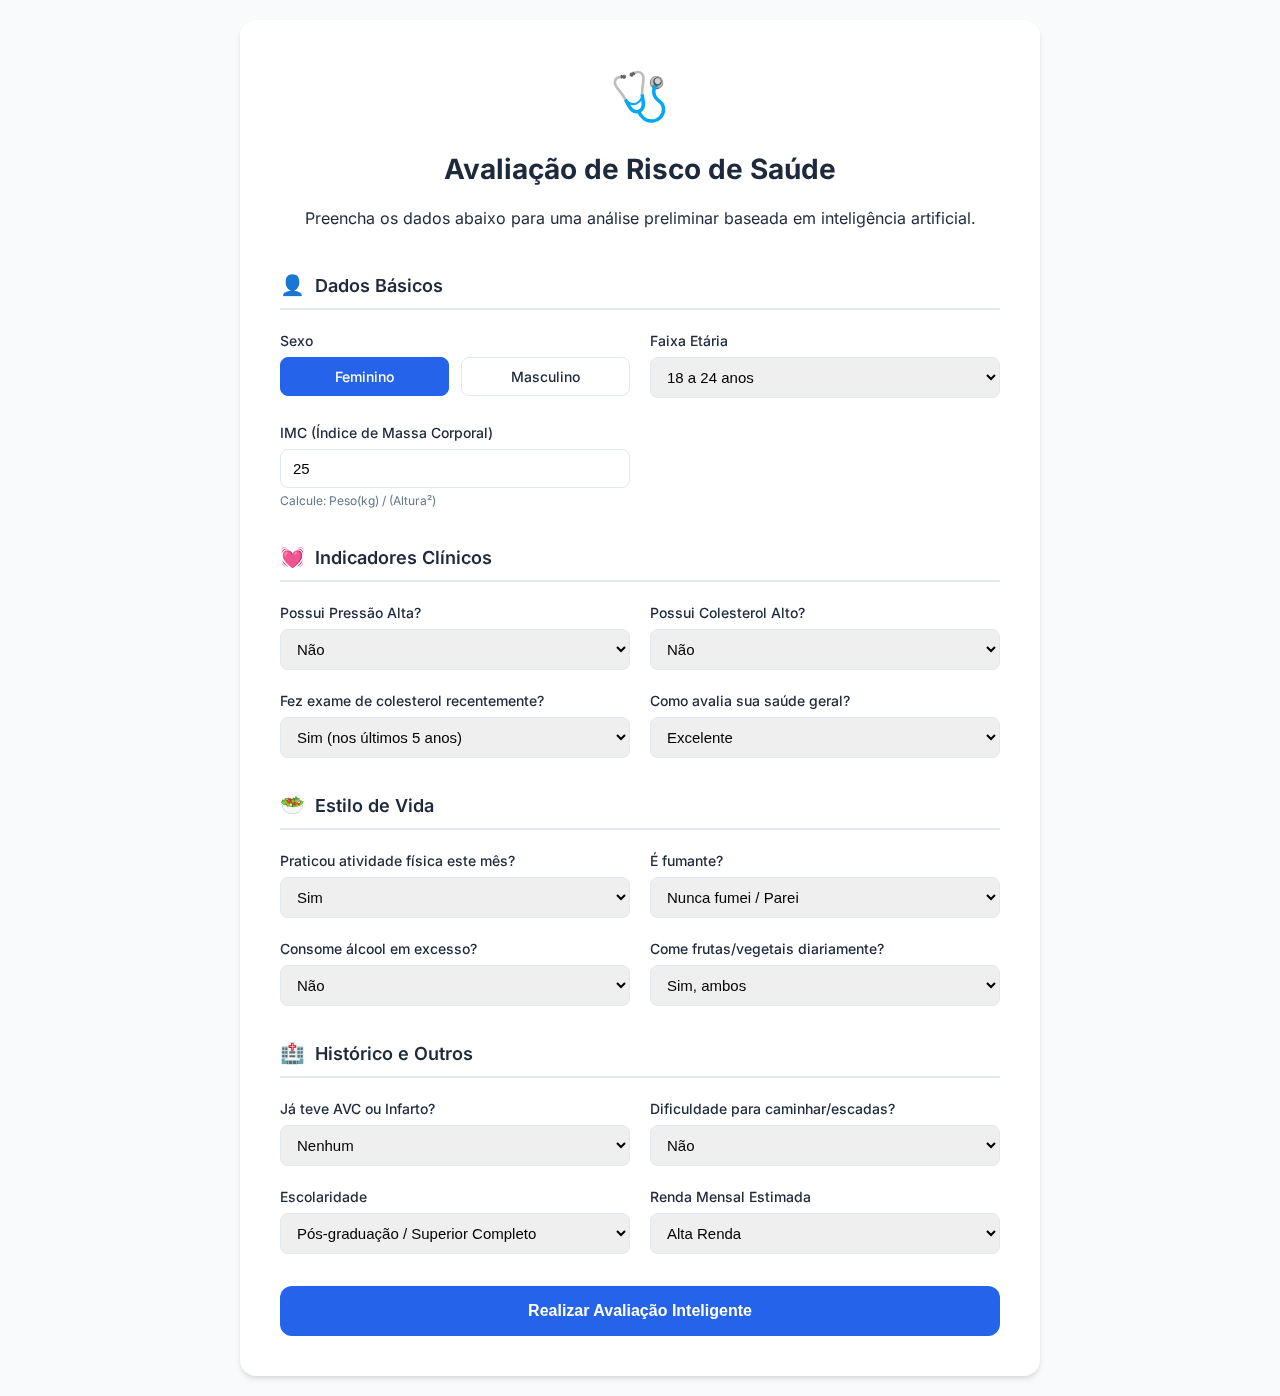
\includegraphics[width=14cm, keepaspectratio]{app_screenshot.png}
\caption{Interface do sistema de infer\^encia web desenvolvido, ilustrando a simplifica\c{c}\~ao do question\'ario para o p\'ublico geral.}
\end{figure}

Alinhado aos resultados das curvas Precision-Recall e da matriz de confus\~ao, que revelaram uma voca\c{c}\~ao do modelo para o rastreio inicial em vez de diagn\'ostico definitivo, a interface foi desenhada para emitir alertas de risco e aconselhar a procura de um profissional de sa\'ude.

\section{Considerações Finais}\label{discussao-e-consideracoes-finais}

Este trabalho explorou o uso de redes neurais profundas (MLP) para a predi\c{c}\~ao de risco de diabetes tipo 2 com base em dados de inqu\'eritos populacionais de sa\'ude. Atingindo uma acur\'acia global de 85,31\%, o modelo apresentou um desempenho aceit\'avel para ser empregado como um instrumento inicial de triagem de baixo custo. A sua principal utilidade pr\'atica reside na capacidade de funcionar como um alerta, facilitando a identifica\c{c}\~ao e a sele\c{c}\~ao de grupos de risco para posterior encaminhamento a exames cl\'inicos e laboratoriais detalhados.

Contudo, a principal limita\c{c}\~ao desta abordagem adv\'em da pr\'opria natureza dos dados autorreportados, que s\~ao inerentemente suscet\'iveis a vieses de mem\'oria e \`a subjetividade do usuário. Isto restringe a precis\~ao metodol\'ogica do sistema se encarado como um fim em si mesmo. Al\'em disso, devido ao natural desequil\'ibrio da base de dados epidemiol\'ogica, o classificador tende a favorecer a classe majorit\'aria, estando sujeito a uma maior taxa de falsos negativos para subgrupos com suscetibilidade gen\'etica e cl\'inica n\~ao mapeadas pelo question\'ario do BRFSS. 

Diante destas fragilidades, e de forma a evoluir a aplica\c{c}\~ao, trabalhos futuros devem investigar uma abordagem multimodal que integre estes dados comportamentais e demogr\'aficos a registos eletr\'onicos de sa\'ude (EHR) geridos por profissionais cl\'inicos, visando aumentar a robustez e a confian\c{c}a m\'edica nas predi\c{c}\~oes.

\section{Disponibilidade de dados e código}\label{disponibilidade-de-dados-e-cuxf3digo}
O código do núcleo de treino e os arquivos da aplicação web estão disponíveis nos repositórios GitHub do projeto (\url{https://github.com/danroxha/diabets} e \url{https://github.com/danroxha/diabets-app}).

\section{Referências bibliográficas}\label{referuxeancias-bibliogruxe1ficas}

\begin{enumerate}

\def\labelenumi{\arabic{enumi}.}

\tightlist

\item TEBOUL, Alex. \emph{Diabetes Health Indicators Dataset}. Kaggle, 2015. Disponível em: https://www.kaggle.com/datasets/alexteboul/diabetes-health-indicators-dataset
\item ABADI, M., et al. \emph{TensorFlow: A system for large-scale machine learning}. OSDI, 2016.
\item XIE, Z., et al. \emph{Building Risk Prediction Models for Type 2 Diabetes Using Machine Learning Techniques}. Journal of Healthcare Engineering, 2019.
\item World Health Organization (WHO). \emph{Global Report on Diabetes}. 2016.
\item GOODFELLOW, I.; BENGIO, Y.; COURVILLE, A. \emph{Deep Learning}. MIT Press, 2016.
\item DANROXHA. \emph{Diabetes Health Indicators - MLP Training Core}. GitHub, 2026.
\item DANROXHA. \emph{Diabetes Risk Predictor App}. GitHub, 2026.
\end{enumerate}


\end{document}
